For the estimation of the azimuth and elevation of a target's position, the phase array radar has been a popular choice during the past decades. This technique employs a series of antennas to transmit and receive the electromagnetic waveform before mentioned. Here, the phase of each element in the group of transmitted is adjusted for the radar to be able to suppress the response from specific directions and thus, "scan" a specific direction. The angular resolution of this method, however, strongly depends on the number of elements in the antenna array. An attractive alternative to the simple phase array is its combination with the \ac{mimo} concept \cite{fishler_mimo_2004}. 

As the name implies, a \ac{mimo} radar consists of multiple transmit (TX) antennas and receive (RX) antennas. $M_t$ transmit and $M_r$ receive elements are assumed. The difference from the phase array radar is that the signals transmitted by each of the TX elements are diversified, leading to $M_t\times M_r$ propagation channels. This, with only $M_t + M_r$ antenna elements. With this concept, a higher performance with a substantially lower cost can be achieved, which is why the \ac{mimo} array has been chosen for the purpose of this thesis. 

Several methods to the define the diversity of the TX channels have been proposed, these include frequency division multiplexing, spatial coding, orthogonal waveforms and time division multiplexing. The latter has been chosen and implemented as presented in \cite{huang_fmcw_2011}. As the name indicates and as presented in \cref{fig:tdm}, the concept time division multiplexing consists in switching the transmit antenna at each consecutive pulse. Hereby, one is able to differentiate at the receiver from which TX element is the signal coming simply by looking at the time of reception, which is important for the estimation of the azimuth profile (\cref{bs:azimuth}).


\begin{figure}[h!]
	\centering
	\begin{tikzpicture}
% Reference Grid
%\draw[gray,very thin] (0,0) grid (10,4); 

%horizontalaxis
\draw[->] (0,0) -- (10,0) node[anchor=north] {$t$}; 
\draw[->] (0,2) -- (10,2) node[anchor=north] {$t$}; 


% t = 0
\draw[dotted] (1,4) --(1,-0.5) node[anchor = west] {$t = 0$}; 
\draw[dotted] (3,-0.5)--(3,4); 
\draw[dotted] (5,-0.5)--(5,4); 
\draw[dotted] (7,-0.5)--(7,4); 
\draw[dotted] (9,-0.5)--(9,4); 

%signals
\draw[blue] (1,0)--(3,1.5); 
\draw[blue] (3,1.5)--(3,0); 
\draw[red] (3,2)--(5,3.5); 
\draw[red] (5,3.5)--(5,2); 
\draw[blue] (5,0)--(7,1.5); 
\draw[blue] (7,1.5)--(7,0); 
\draw[red] (7,2)--(9,3.5); 
\draw[red] (9,3.5)--(9,2); 
\draw[blue] (9,0)--(10,0.75); 


%Distances
\draw[<->] (1,3.5)--(3,3.5); 
\draw (2,3.7) node {$T_c$}; 

%labels
\draw(0,0.3) node {TX1}; 

\draw(0,2.3) node {TX2};



\end{tikzpicture}
	\caption{Time division multiplexing for \Ac{mimo}-radar.}
	\label{fig:tdm}
\end{figure} 


A further design concern is the array manifold. Different array forms can be found in literature, where the most common are the uniform linear array (ULA) and the uniform circular array (UCA) \cite{zhang_blind_2009}, which are depicted in \cref{fig:ula,fig:uca}. As the name indicates, this manifolds consists of equidistant antenna elements in either linear or circular form. The MIMO-radar chosen here consists in 2 TX and 4 RX array resulting in 8 virtual channels.

\begin{figure}[h!]
	\centering
	\begin{minipage}{.5\textwidth}
		\centering
		\begin{tikzpicture}
% Reference Grid
\draw[white,very thin] (0,0) grid (5,5); 

   \tikzstyle{tx} = [draw, shape=rectangle, minimum height=0.1cm, minimum width=0.1cm, node distance=0.0005cm and 0.0005cm, line width=1pt, fill = blue]
\tikzstyle{rx} = [draw, shape=rectangle, minimum height=0.1cm, minimum width=0.1cm, node distance=0.0005cm and 0.0005cm, line width=1pt, fill = red]
\tikzstyle{virt} = [draw, shape=rectangle, minimum height=0.1cm, minimum width=0.1cm, node distance=0.0005cm and 0.0005cm, line width=1pt, fill = black]
\draw[dotted] (0,1)--(4.5,4); 
\draw[->] (0,1) -- (6,1) node[anchor=north] {$x$}; 
\draw[->] (0,1) -- (0,4) node[anchor=east] {$y$}; 

\node at (0,1) [tx, label = below: \footnotesize $0$] (){}; 
\node at (1,1) [tx, label = below: \footnotesize $d$] (){}; 
\node at (2,1) [tx, label = below: \footnotesize $2d$] (){}; 
\node at (5,1) [tx, label = below: \footnotesize $(L-1)d$] (){}; 

\draw[black, fill = black] (3,3) circle(0.1cm);
\node at (3,3) [anchor = north] {\footnotesize Target}; 



 \draw (0,1.7) arc (90:48:1);
\node at (0.4,2.3) [label = below: \footnotesize $\theta$](){}; 
\end{tikzpicture}

		\captionof{figure}{Uniform Linear Array (ULA).}
		\label{fig:ula}
	\end{minipage}%
	\begin{minipage}{.5\textwidth}
		\centering
		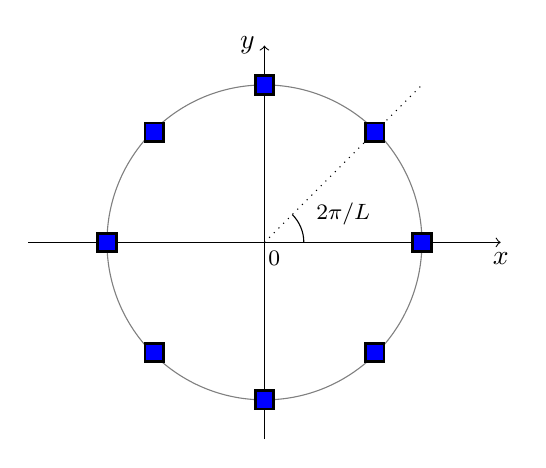
\begin{tikzpicture}
% Reference Grid
\draw[white,very thin] (0,0) grid (5,5); 

   \tikzstyle{tx} = [draw, shape=rectangle, minimum height=0.1cm, minimum width=0.1cm, node distance=0.0005cm and 0.0005cm, line width=1pt, fill = blue]
\tikzstyle{rx} = [draw, shape=rectangle, minimum height=0.1cm, minimum width=0.1cm, node distance=0.0005cm and 0.0005cm, line width=1pt, fill = red]
\tikzstyle{virt} = [draw, shape=rectangle, minimum height=0.1cm, minimum width=0.1cm, node distance=0.0005cm and 0.0005cm, line width=1pt, fill = black]


\draw[dotted] (3,2.5)--(5,4.5); 

\draw[->] (0,2.5) -- (6,2.5) node[anchor=north] {$x$}; 
\draw[->] (3,0) -- (3,5) node[anchor=east] {$y$}; 

\node at (2.8,2.3) [ label = right: \footnotesize $0$] (){}; 

\draw[gray](3,2.5)circle(2.0cm); 

 \draw (3.5,2.5) arc (0:45:0.5);
 \node at (4,3.25) [label = below: \footnotesize $2\pi/L$](){}; 


\node at (3,4.5)[tx](){}; 
\node at (3,0.5)[tx](){};
\node at (1,2.5)[tx](){};
\node at (5,2.5)[tx](){};   
\node at (1.6,3.9)[tx](){};
\node at (4.4,3.9)[tx](){};
\node at (1.6,1.1)[tx](){};
\node at (4.4,1.1)[tx](){};

\end{tikzpicture}

		\captionof{figure}{Uniform Circular Array (UCA).}
		\label{fig:uca}
	\end{minipage}
\end{figure}

If the far-field condition is satisfied, the \Ac{mimo}-configuration can be modeled as an ULA of  $M_t\times M_r$ virtual antennas. Given the position of the TX-elements $x_i^{Tx}$ and RX-elements $x_j^{Rx}$ the virtual ULA is modeled by antenna elements at 

\begin{equation}
\vec{x_{ij}} = (\vec{x}_i^{Tx}+\vec{x}_j^{Rx})/2\\,
\end{equation}
for $i = 1,...,M_t$ and $j = 1,...,M_r$. Presented in \cref{fig:mimo_array} is a \Ac{mimo}-setup with its corresponding virtual elements. Note that for this work the TX and RX elements are aligned in the vertical axis. This has been ignored here for better illustration. 

\begin{figure}[h]
	\centering
	A \ac{mimo} setup for this research has been chosen. The concepts behind the \ac{mimo} radar will be presented briefly in this section. 

As the name implies, a \ac{mimo} radar consists of multiple transmit (TX) antennas and receive (RX) antennas. Given $M_t$ transmit and $M_r$ receive elements in an array, $M_t\times M_r$ propagation channels are obtained. This, with only $M_t
M_r$ antenna elements. Furthermore, a method to define the diversity of the TX channels is required. This can be achieved by employing time division multiplexing, frequency division multiplexing, spatial coding, and orthogonal waveforms \cite{huang_fmcw_2011}. 

Each of the  $M_t\times M_r$ propagation channels are modeled together as a virtually form array. Each element in the virtual array is placed at 
\begin{equation}
	\vec{x_{ij}} = (\vec{x}_i^{Tx}+\vec{x}_j^{Rx})/2\\,
\end{equation}
where $\vec{x}_i^{Tx}$ is the position of the $i$-TX element and $\vec{x}_j^{Rx}$ of the $j$-RX element, as shown in \cref{fig:mimo_array}

\begin{figure}[h]
	\centering
	A \ac{mimo} setup for this research has been chosen. The concepts behind the \ac{mimo} radar will be presented briefly in this section. 

As the name implies, a \ac{mimo} radar consists of multiple transmit (TX) antennas and receive (RX) antennas. Given $M_t$ transmit and $M_r$ receive elements in an array, $M_t\times M_r$ propagation channels are obtained. This, with only $M_t
M_r$ antenna elements. Furthermore, a method to define the diversity of the TX channels is required. This can be achieved by employing time division multiplexing, frequency division multiplexing, spatial coding, and orthogonal waveforms \cite{huang_fmcw_2011}. 

Each of the  $M_t\times M_r$ propagation channels are modeled together as a virtually form array. Each element in the virtual array is placed at 
\begin{equation}
	\vec{x_{ij}} = (\vec{x}_i^{Tx}+\vec{x}_j^{Rx})/2\\,
\end{equation}
where $\vec{x}_i^{Tx}$ is the position of the $i$-TX element and $\vec{x}_j^{Rx}$ of the $j$-RX element, as shown in \cref{fig:mimo_array}

\begin{figure}[h]
	\centering
	A \ac{mimo} setup for this research has been chosen. The concepts behind the \ac{mimo} radar will be presented briefly in this section. 

As the name implies, a \ac{mimo} radar consists of multiple transmit (TX) antennas and receive (RX) antennas. Given $M_t$ transmit and $M_r$ receive elements in an array, $M_t\times M_r$ propagation channels are obtained. This, with only $M_t
M_r$ antenna elements. Furthermore, a method to define the diversity of the TX channels is required. This can be achieved by employing time division multiplexing, frequency division multiplexing, spatial coding, and orthogonal waveforms \cite{huang_fmcw_2011}. 

Each of the  $M_t\times M_r$ propagation channels are modeled together as a virtually form array. Each element in the virtual array is placed at 
\begin{equation}
	\vec{x_{ij}} = (\vec{x}_i^{Tx}+\vec{x}_j^{Rx})/2\\,
\end{equation}
where $\vec{x}_i^{Tx}$ is the position of the $i$-TX element and $\vec{x}_j^{Rx}$ of the $j$-RX element, as shown in \cref{fig:mimo_array}

\begin{figure}[h]
	\centering
	\input{fundamentals_figs/mimo.tex}
	\caption{\ac{mimo}-array}
		\label{fig:mimo_array}
\end{figure} 

 If the far-field condition is met for a given scatterer at position $\vec{p}$, the signal propagation path from a given TX element to the scatterer, plus the reflection path back to an RX element can be approximated as
 \begin{equation}
 	P_{ij}(p) = |\vec{p}-\vec{x}_i^{Tx}| + |\vec{p}-\vec{x}_j^{Rx}| \approx 2|\vec{p}-\vec{x}_{ij}| 
 \end{equation}
	\caption{\ac{mimo}-array}
		\label{fig:mimo_array}
\end{figure} 

 If the far-field condition is met for a given scatterer at position $\vec{p}$, the signal propagation path from a given TX element to the scatterer, plus the reflection path back to an RX element can be approximated as
 \begin{equation}
 	P_{ij}(p) = |\vec{p}-\vec{x}_i^{Tx}| + |\vec{p}-\vec{x}_j^{Rx}| \approx 2|\vec{p}-\vec{x}_{ij}| 
 \end{equation}
	\caption{\ac{mimo}-array}
		\label{fig:mimo_array}
\end{figure} 

 If the far-field condition is met for a given scatterer at position $\vec{p}$, the signal propagation path from a given TX element to the scatterer, plus the reflection path back to an RX element can be approximated as
 \begin{equation}
 	P_{ij}(p) = |\vec{p}-\vec{x}_i^{Tx}| + |\vec{p}-\vec{x}_j^{Rx}| \approx 2|\vec{p}-\vec{x}_{ij}| 
 \end{equation}
	\caption{\ac{mimo}-array}
		\label{fig:mimo_array}
\end{figure} 
 
 Under the described conditions the signal propagation path from a given TX element to a scatterer at point $\vec{p}$, plus the reflection path back to an RX element can be approximated as
 \begin{equation}
 	P_{ij}(p) = |\vec{p}-\vec{x}_i^{Tx}| + |\vec{p}-\vec{x}_j^{Rx}| \approx 2|\vec{p}-\vec{x}_{ij}| \\.
 \end{equation}